% !TeX encoding = UTF-8
% Use XeLaTeX to compile it
%
% Эта работа распространяется на условиях лицензии Creative Commons Attribution-Noncommercial-Share Alike 3.0 New Zealand License.
% Краткое описание лицензии есть тут: http://creativecommons.org/licenses/by-nc-sa/3.0/nz/deed.ru
% Полное — там же.
% Эту книгу можно невозбранно распространять и изменять, но только соблюдая следующие условия:
% сохраняя лицензию и не вводя дополнительных ограничений, бесплатно
% и указывая авторство как оригинальной части, так и изменённой.
% Автор оригинального английского текста — Jason R Briggs http://jasonrbriggs.com/
% Автор перевода — Егор Кочетов <Egor.Kochetoff@gmail.com>
%
% This work is licensed under the Creative Commons Attribution-Noncommercial-Share Alike 3.0 New Zealand License.
% To view a copy of this license, visit http://creativecommons.org/licenses/by-nc-sa/3.0/nz
% or send a letter to Creative Commons, 171 Second Street, Suite 300, San Francisco, California, 94105, USA.
%

\chapter{Не все змеи будут шипеть на тебя}\label{ch:notallsnakeswillsquishyou}

Возможно, тебе подарили эту книгу на день рожденья. А может, на рождество. Например, так: тётя Агата (у всех есть тётя Агата, но не все об этом знают) хотела подарить носки, хотя и не парные, но оба красивые, на два размера больше — на вырост (и всё равно бы эти носки не пригодились потом). А потом вместо этого услышала про эту книгу (которую можно взять и напечатать), вспомнила твои вопросы про всякие компьютерные штуки, и твои непонятные объяснения, как пользоваться компьютером, оборвавшиеся в момент, когда она начала разговаривать с компьютерной мышью, и решила подарить эту книгу. Во всяком случае эта книга уж точно лучше пары разных носков.

Надеюсь, я не слишком тебя разочаровываю тем, что я — возможно, напечатанная на какой-нибудь старой обёрточной бумаге (хотя если повезло, то и нет) — не слишком разговорчивая (прямо, скажем, совсем молчаливая) книга, с пугающим словом «изучение» в названии... Но представь на минутку и мои ощущения. Если бы вот ты был персонажем из какой-нибудь книги про волшебников, одна из которых наверняка есть у тебя в спальне на книжной полке, — у меня бы могли быть зубы... или даже глаза! А ещё какие-нибудь движущиеся картинки, таинственные звуки... ладно, чего я. В общем, я просто бумажная книжка, хотя могло бы быть и лучше.

\btw{Ах, много бы я дала за пару хороших острых челюстей...}

Но вообще, быть конкретно такой книжкой тоже не слишком печально. Ну не могу я говорить... пальцы покусывать не могу; зато могу рассказать немного о том, что заставляет компьютеры работать. Не про разные аппаратные штуки — все эти провода, платы, чипы — они меня немного пугают. Электричеством, например, могут ударить (так что не стоит и пытаться туда лезть, как по мне). Я могу рассказать о том, что удивительным образом скрыто внутри всех этих проводов, микросхем и что делает компьютер по-настоящему полезным.

\begin{wrapfigure}{r}{0.5\textwidth}
  \begin{center}
\includegraphics*[width=70mm]{../en/electrocute.eps}
  \end{center}
\end{wrapfigure}

Вообще, это здорово похоже на мысли, например, в твоей голове. Если бы мыслей у тебя не было — сидел бы ты, скажем, на полу в спальне и бессмысленно смотрел в пространство перед собой. Без \emph{программ} компьютеры бы могли приносить пользу, пожалуй, разве что как стопор для двери. Да и то посредственный: вечно все бы об него спотыкались по ночам. А что может быть хуже, чем удариться ночью в темноте пальцем ноги с размаху о железный угол...

\btw{Итак, я всего лишь книга. И мне это хорошо известно.}

У тебя в семье могут быть разные устройства вроде Playstation, Xbox, Wii — игровые консоли, — а ещё DVD-проигрыватель, может, даже современный холодильник и игрушечная машинка. В них во всех есть программы, которые делают их намного полезнее, чем если бы эти штуки были без программ. В DVD-проигрывателе есть программа для чтения и воспроизведения дисков. В холодильнике — какая-то простая программа для поддержания температуры при минимальных затратах электричества. В машинке — программа для приёма команд с пульта управления и для езды в ответ на эти команды. А в настоящих машинах программы показывают маршруты в объезд пробок и сигналят водителю, когда он паркуется, чтоб он никуда не въехал (в стену или соседнюю машину).

Зная, как писать программы, ты сможешь сделать множество самых разных полезных вещей. Можно свою игру написать. Можно писать страницы в интернете, которые что-нибудь делают, а не просто показывают текст и картинки. Можно упрощать себе выполнение домашней работы.

Так вот, пора приступить к чему-то чуть более интересному, чем эти рассуждения.

\section{Пара слов про язык}

Так же как и у людей, определённо как у китов, возможно, и у дельфинов и, возможно, у родителей (тут, конечно, спорно), у компьютеров есть свой собственный язык. Вообще, как и у людей, у компьютеров много языков. Какую букву английского алфавита ни возьми, она называет какой-нибудь язык. Вот, например, буквы A, B, C, D, E — не только буквы, но и названия языков программирования (что ещё раз доказывает, что у взрослых никакого воображения и хорошо бы им давать почитать хотя бы словарь перед тем, как названия придумывать).

Есть ещё языки программирования, названные в честь людей\footnote{например, язык Ада — в честь \href{https://ru.wikipedia.org/wiki/\%D0\%9B\%D0\%B0\%D0\%B2\%D0\%BB\%D0\%B5\%D0\%B9\%D1\%81,_\%D0\%90\%D0\%B4\%D0\%B0}{Ады Лавлейс}. А есть ещё язык \href{https://ru.wikipedia.org/wiki/\%D0\%A3\%D1\%87\%D0\%B5\%D0\%B1\%D0\%BD\%D1\%8B\%D0\%B9_\%D0\%B0\%D0\%BB\%D0\%B3\%D0\%BE\%D1\%80\%D0\%B8\%D1\%82\%D0\%BC\%D0\%B8\%D1\%87\%D0\%B5\%D1\%81\%D0\%BA\%D0\%B8\%D0\%B9_\%D1\%8F\%D0\%B7\%D1\%8B\%D0\%BA}{РАЯ}.},
есть языки-сокращения из заглавных букв (SQL, например),  есть немножко названных в честь телевизионных шоу. А, да, ещё если дописать к этим буквам всяких значков типа плюсиков, решёточек (+, \#), то тоже получатся названия разных языков программирования. И ещё впридачу некоторые языки очень похожи и отличаются только в каких-то мелочах.

\btw{Что я говорила? Никакого воображения!}

К счастью, многие из языков уже почти не используются или совсем исчезли; но однако же список способов «говорить» с компьютером всё ещё пугающе велик. Я буду обсуждать только один из них, потому что иначе всё так и закончится их перечислением, не успеем мы приступить к чему-то действительно интересному.

\section{Орден Неядовитых Удушающих Змей...}

... или просто питонов.

Вообще, питон — не только змея\footnote{которая \href{https://ru.wikipedia.org/w/index.php?title=\%D0\%9F\%D0\%B8\%D1\%82\%D0\%BE\%D0\%BD\%D1\%8B&oldid=70828612\#.D0.9F.D0.B8.D1.82.D0.B0.D0.BD.D0.B8.D0.B5}{может} не есть полтора года кряду!}, но и язык программирования. Многие называют его «пайтон», как принято за рубежом, где его и придумали (и пишут его название как Python). Язык, правда, был назван не в честь змеи — это один из немногих языков программирования, названных в честь телевизионного шоу. \href{http://www.youtube.com/watch?v=YO2xZbac7lw&list=PL89E217812DCA2BDA}{Монти Пайтон} (Monty Python) — \href{http://www.montypython.com/}{британское телешоу}, популярное с 1970х годов. Требуется достичь некоторого возраста и иметь определённый склад ума, чтобы счесть его забавным, но многим нравится. Хотя лет до 12 смотреть вообще смысла нет, будет скучно и непонятно.

Есть несколько особенностей Питона (языка программирования, а не змеи), делающих его очень полезным, чтобы учиться программировать. Для нас сейчас важнее всего то, что используя его, можно быстро сесть и начать писать какие-то программки, пусть и очень простые, без долгих разговоров и объяснений.

Это тот момент, когда надо убедиться, что твоя мама, папа или кто там управляет компьютером прочли часть «Заметка для мам и пап».
\begin{WINDOWS}
Если что-то не получится, надо спешить к ним за помощью.

Нажми на кнопку «Пуск» (она обычно слева внизу на экране), потом напечатай слово «Python». Должен появиться значок командной строки (чёрный квадратик с белой каймой) с названием «Python», «Python 3.5» или каким-то похожим. На рисунке \ref{fig1} показано, как это может выглядеть. Нужно запустить программу, которая называется «Python (командная строка)», «Python (command line)» или как-нибудь вроде этого. В результате должно появиться окно, как на рисунке \ref{fig2}.

\begin{figure}
	\begin{center}
		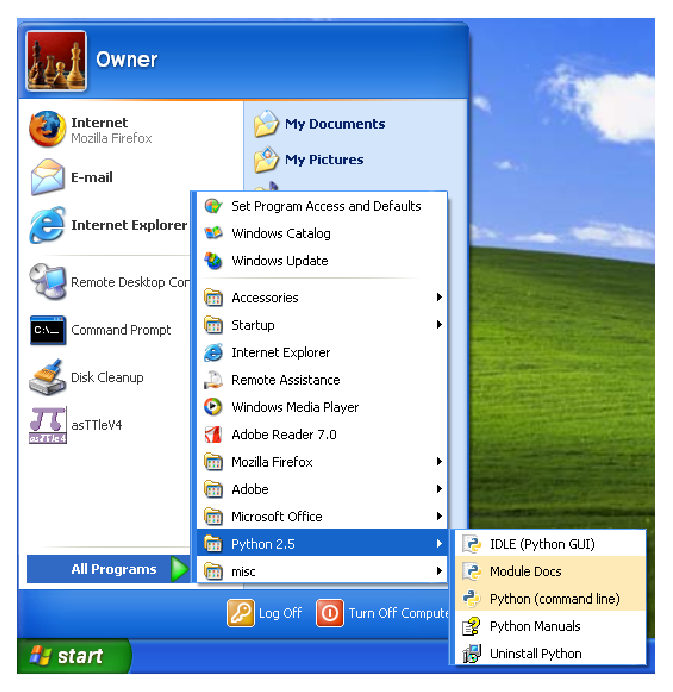
\includegraphics[width=80mm]{../en/figure1.eps}
	\end{center}
	\caption{Python в меню Windows.}\label{fig1}
\end{figure}

\begin{figure}
	\begin{center}
		
\includegraphics[width=135mm]{../en/figure2.eps}
	\end{center}
	\caption{Консоль Питона в Windows.}\label{fig2}
\end{figure}
\end{WINDOWS}
\begin{MAC}
%TODO перевести на русский (у меня нет Mac'а)
В программе Finder слева есть категории, одна из которых называется «Applications». Нажми на неё и найди там программу, которая называется «Terminal» (она часто находится в папке «Utilities»). Нажми на значок терминала, а когда он запустится, введи туда слово «python» (маленькими буквами) и нажми на клавиатуре Enter. Если всё прошло как надо, то на экране появится окно, как на рисунке \ref{fig3}.

\begin{figure}
	\begin{center}
		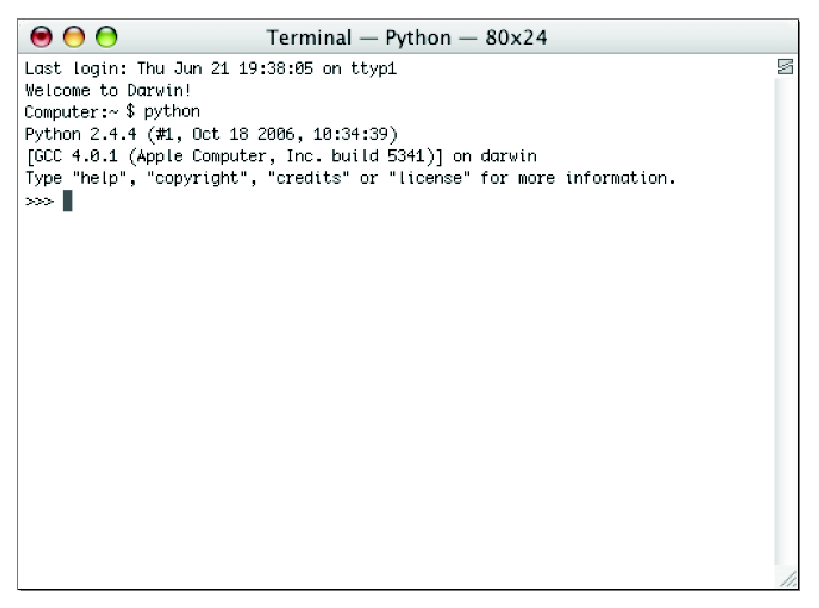
\includegraphics[width=85mm]{../en/figure3.eps}
	\end{center}
	\caption{Консоль Питона в Mac OS X.}\label{fig3}
\end{figure}
\end{MAC}
\begin{LINUX}
Есть хороший способ проверить это. Спроси у них, как называется программа-\emph{эмулятор терминала} — это может быть \texttt{yakuake}, \texttt{konsole}, \texttt{rxvt}, \texttt{xterm} или ещё какая-нибудь, их очень много бывает — именно поэтому придётся спросить. Запусти эту программу, напиши \emph{в командной строке} «python3» (без кавычек) и нажми на клавиатуре клавишу Enter. На экране должно появиться что-то похожее на рисунок \ref{fig4}.

\begin{figure}
\begin{center}
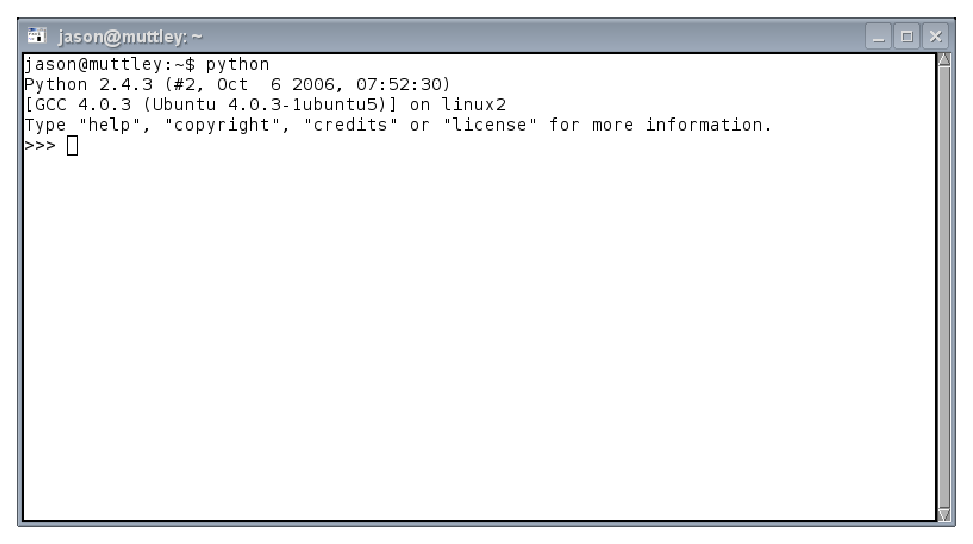
\includegraphics[width=80mm]{../en/figure4.eps}
\end{center}
\caption{Консоль Питона в Линуксе.}\label{fig4}
\end{figure}
\end{LINUX}

\begin{samepage}
\note{Если ты обнаружишь, что родители не прочитали инструкции в начале книги...}
\nopagebreak
\paragraph*{}
... и из-за этого у тебя не получилось что-то сделать, то перелистни эту книгу на начало, подсунь им под нос введение, пока они читают утреннюю газету, и умоляюще посмотри на них. Иногда помогает говорить «пожалуйста-пожалуйста-пожалуйста» до тех пор, пока они не встанут и не сделают всё, что надо. Ну и конечно, можно попробовать сделать всё самостоятельно, это может оказаться даже проще.
\end{samepage}

\section{Первая программа на Питоне}

Так или иначе, если ты добрался досюда, у тебя уже открыта \emph{консоль}, или командная строка Питона — это один из способов запускать команды и целые программы на Питоне. После запуска консоли или ввода любой команды ты увидишь \emph{приглашение командной строки}, которое в Питоне выглядит вот так:

\begin{verbatim}
>>>
\end{verbatim}

Если записать несколько команд на Питоне одну за другой, получится программа, которую можно запускать и не через консоль, но пока на минутку остановимся на простых командах, которые можно вводить прямиком в командную строку (после «приглашения»). Например, можно ввести туда следующую команду:

\begin{verbatim}
print("Всем привет!")
\end{verbatim}

Чтобы всё получилось, нужно ввести и скобки и кавычки (вот эти: "") так, как написано выше. Тогда на экране должно появиться что-то вроде такого:

\begin{verbatim}
>>> print("Всем привет!")
Всем привет!
\end{verbatim}

После этого приглашение командной строки появится снова, чтобы показать, что Питон готов принимать новые команды. Поздравляю! Ты только что создал и запустил свою первую программу на Питоне — пусть пока и всего из одной команды: print — функции, которая просто печатает всё, что написано в скобках. Потом мы много будет использовать эту команду.

\section{Вторая программа на питоне… опять то же самое?}

Программы на Питоне были бы не слишком полезными, если бы их приходилось каждый раз вводить заново в командную строку или если бы ты написал программу для кого-то, а ему бы пришлось её перепечатывать, чтобы запустить.

Программа для редактирования текстов (Microsoft Word, Libreoffice Writer или другая подобная), которую ты, вероятно, используешь для выполнения каких-нибудь домашних заданий, получена из исходного кода размером примерно от 10 до 100 миллионов строк. Если печатать это на бумаге с двух сторон не очень крупно, это может занять, например, 400 000 страниц. Это стопка бумаги высотой 40 метров, с десятиэтажный дом. Такое количество бумаги нести из магазина в дом, чтобы перепечатать, пришлось бы долго… очень долго…

…а если бы ещё и ветер подул в подходящий момент… за бумагой пришлось бы долго бегать. Так вот, хорошая новость: всем этим заниматься не обязательно.

\begin{center}
\includegraphics*[width=85mm]{../en/pullinghair.eps}
\end{center}

\begin{WINDOWS}
Открой Блокнот (например, так: нажми «Пуск» и напечатай «блокнот») и введи туда команду в точности так, как она напечатана ниже, как до этого мы вводили её в консоль:

\begin{listing}
\begin{verbatim}
print("Всем привет!")
\end{verbatim}
\end{listing}

Нажми в блокноте на меню «Файл», выбери там пункт «Сохранить» и сохрани этот файл под именем \emph{hello.py} на рабочем столе. Теперь запусти (двойным щелчком) этот файл с рабочего стола. На секунду мелькнёт чёрное окно консоли. В это может быть трудно поверить, но там как раз напечатано то, о чём мы просили. Пока в этом можно убедиться, сделав быстро снимок экрана, пока окно не пропало, и разглядев это на снимке, но я на этом останавливаться не буду. Позже мы вернёмся к нашему коду и убедимся, что всё и правда печатается как надо, не применяя ловкости рук.

\begin{figure}
	\begin{center}
		
\includegraphics[width=58mm]{../en/figure5.eps}
	\end{center}
	\caption{Значок hello.py на рабочем столе Windows.}\label{fig5}
\end{figure}
\end{WINDOWS}

\begin{MAC}
%TODO перевести про Mac
Открой текстовый редактор, нажав на его значок. Он может быть на панели внизу экрана, вот такой: \includegraphics*[width=12mm]{../en/textedit-icon.eps}; или ещё его можно поискать в списке Applications в Finder'е, такой: \includegraphics*[width=19mm]{../en/textedit-icon2.eps}. Введи туда ту же команду для печати, что мы ввели только что в консоль:

\begin{listing}
	\begin{verbatim}
	print("Всем привет!")
	\end{verbatim}
\end{listing}

Теперь открой вверху меню файл, выбери «сохранить» и сохрани этот файл в домашнюю папку под именем «hello.py». После этого опять открой терминал (он как раз открывается в домашней директории) и запусти наш скрипт:

\begin{listing}
	\begin{verbatim}
	python hello.py
	\end{verbatim}
\end{listing}

Результат должен быть такой же, как и раньше, когда мы вводили команду прямо в консоль Питона.
\end{MAC}

\begin{LINUX}
Открой текстовый редактор (можешь опять спросить у родителей, как он называется: например, kate, gedit, kdevelop, но никак не OpenOffice Write, он не подойдёт) и напиши туда точно ту же самую команду, что мы до этого вводили в консоль:

\begin{verbatim}
print("Всем привет!")
\end{verbatim}

%todo save.png
Теперь сохрани этот файл в своей домашней папке. Наверху в программе должен быть значок сохранения, а когда тебя спросят, куда сохранять, нажми на какую-нибудь кнопку типа домика. В качестве имени файла введи «hello.py». Теперь опять открой терминал и напиши:

\begin{verbatim}
python hello.py
\end{verbatim}

В консоли должно появиться приветствие от программы, точно так же, как в прошлый раз (примерно как на рисунке \ref{fig9}).

\begin{figure}
\begin{center}

\includegraphics[width=75mm]{../en/figure9.eps}
\end{center}
\caption{Запуск программы на Питоне, сохранённой в текстовый файл}\label{fig9}
\end{figure}
\end{LINUX}

Вот. Теперь ты видишь, что мудрые люди, создавшие Питон, спасли тебя от ввода одних и тех же программ много-много-много раз для выполнения одних и тех же действий. Как они делали в 1980х. Я серьёзно, им приходилось вводить каждый раз кучу команд для выполнения одной и той же программы. Можешь спросить у папы — вдруг у него был ZX81 в молодости — так там приходилось так делать. Теперь можно просто написать имя программы, и она целиком исполнится от начала до конца.

\note{Конец начала}

Добро пожаловать в удивительный мир программирования!
Мы начали с простой программы, которая печатает «Всем привет» («Hello world») — все с этого начинают, когда учатся программировать. В следующей главе мы займёмся чуть более полезными вещами в консоли Питона, а потом изучим, как написать программу посложнее.
